\chapter{Computer System Security}
I took this class in the Fall of 2025 with a notably "poor" professor named
Randall "Randy" Klepetko and let me tell you... I really need to stop reading the reviews
about professors on RateMyProfessor because he was anything but "poor". To paint a picture
of Dr. Klepetko, go to a Grateful Dead concert and pick any long haired, maybe late fifty's,
tall skinny dude out of the crowd, and I'd say they might be a spitting image of him. I mean
this in the absolute best way possible; he literally would be at that concert, and it may
very much be him. The reviews said things along the lines of "he's rude to students", or
"his tests are impossible". While I've never heard him be rude to a student, I can say that
the tests were inherently challenging due to the nature of the courses he taught (this one and
Computer Architecture). So main takeaway from this course? Don't believe what you read on the
internet, especially if it's written by a frustrated 18-year-old who couldn't ChatGPT their
way through the course.

So what is this course? It's a very high level of understanding what Computer System Security
is and understanding some of the threats that machines (computers) are exposed to.

\section{Introduction}
\section{Attacks}
\section{Defenses}
What is more challenging; Attacking or Defending a computer? Defending, by far.
To attack a computer, you only need to find one vulnerability; To defend one, you
have to mitigate all vulnerabilities.



\subsection{Monitoring/Detection}
In order to prevent attacks, a system must continuously monitor changes to detect
any potential threats. The system monitors:

\begin{itemize}
    \item Files
    \item Memory
    \item Processes
    \item Input/Output
    \item Disk Activity
\end{itemize}


Each is monitored by two different types of Detection Analysis

\subsubsection{Static Analysis}

\textbf{Static Analysis} is your \textbf{Anti-Virus} or \textbf{file alteration
detection} software. It constantly checks whether there is a \textit{"virus
file"} present on the machine. If one is detected, it immediately puts it into
quarantine to prevent it from making any unauthorized changes. Antivirus
software is \textbf{very effective}, almost 99\% percent of the time it can pick
up these types of files.

I would assume that it's so effective because it has seen thousands and
thousands of different iterations of all the possible file constructs to be able
to detect whether a file is safe. Because of this, Antivirus is ineffective
against \textit{Zero-Day Exploits} \newline

\begin{tcolorbox}[mybox] A \textbf{\textit{Zero-Day Exploit}} is a type of
attack that attempts to inject itself into a brand-new program before the first
patch is released.


\begin{center} 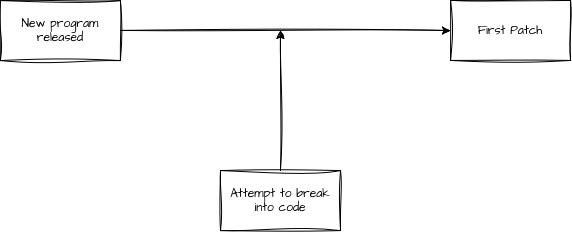
\includegraphics[width=400px]{zero_day} \end{center}

\end{tcolorbox}

\subsubsection{Dynamic Analysis} \textbf{Dynamic Analysis} dynamically checks
whether certain events fall meet a certain set of criteria  of a specified
range, using either the Poisson or Gaussian Distribution. For example, it could
be the number of times a file tries to access a directory whose permissions are
locked. If it tries, say, 100 times, then that would appear as an outlier on
either distribution.  Once this happens, it then quarantines the file to make
sure that if it is indeed a virus, it can't do any more damage.


Because it is running on live \textit{(dynamic data)}, it is not as effective as
Static Analysis because it's "learning as it goes", sort of. While it's not good
as a first line of defense, it's fantastic at detecting \textit{Zero-Day
Exploits.}

\subsubsection{Specification Anomalies}


\subsubsection{Machine Learning}
Machine Learning is used to detect different anomalies.
\subsection{Response and Recovery}
What is the proper course of action when, through either Static or Dynamic Analysis,
to take when a questionable file is detected?

\begin{enumerate}
    \item \textbf{Document} the attack. What happened, where did it come from, etc.
    \item \textbf{Disconnect and Delay}. Try to disconnect the part of the system that caused the attack. If say, the Hard Disk Drive is detected as the source, electronically disconnect that from the rest of the system.
    \item \textbf{Monitor} the system for any further anomalies. I would think that this is a type of monitoring that is on steroids.
    \item \textbf{Isolate} the file/root of the attack and put it's ass in jail. Not literally, but quarantine it so that it can't cause any more damage.
    \item \textbf{Set up a Honeypot} to see if there are any more sneaky bastards hanging around that weren't detected.
    \item \textbf{Misdirect} or set up a trap door for those attacks.
    \item \textbf{Restore and Recover} files that were damaged to an earlier restore point, if possible. Otherwise, tell the user they are silly goose's for not backing up their system and then proceed throw errors.
\end{enumerate}

\begin{tcolorbox}[mybox]
A good procedure to follow is called the \textbf{LOCUS Approach}. The fundamental ideas are
\begin{center}
    \textbf{Establish a security foundation} and \textbf{implement best practice standards.}
\end{center}

\end{tcolorbox}